%
% boundry.tex  -- 
%
% (c) 2019 Prof Dr Andreas Mueller
%
\section{Boundary conditions}
\index{boundary conditions!for quasilinear partial differential equations of first order}
The method of characteristics allows us to find out on which parts of the
boundary we have to specify boundary conditions to make the solution
unique.
The solution surface corresponding to $u(x,y)$ consists of characteristics
so it is uniquely determined if exactly one characteristic goes through
each point.

For the differential equation
\begin{equation}
\frac{\partial u}{\partial x}+2\frac{\partial u}{\partial y}=3
\label{geometrie:knickbeispiel}
\end{equation}
we have found the characteristics
\[
t\mapsto\begin{pmatrix}x_0\\y_0\\z_0\end{pmatrix}+t\begin{pmatrix}1\\2\\3\end{pmatrix}.
\]
The graph of the solution function $u(x,y)$ must be covered by characteristics.
The projections of these curves into the $x$-$y$-plane are straight lines
with slope $2$.
The boundary of the domain $\Omega$, in which the equation needs to be
solved, thus must intersect each straight line with slope $2$ exactly once.

The domain
$\{(x,y)\in\mathbb R^2\,|\, x >0\}$  from \ref{konstantekoeff}
has the $x$-axis as boundary which intersects every straight line with
slope exactly once.

The domain $\Omega=\{(x,y)\,|\,0<x,y<1\}$ is more interesting.
Figures \ref{geometrie:charrand1}
to \ref{geometrie:charrand3}
show various possibilities:
\begin{enumerate}
\item
In figure~\ref{geometrie:charrand1}
boundary values are prescribed on the left and right boundary.
These boundary values are not sufficient to determine the solution
everywhere in the domain.
There is a part not covered by characteristics where the solution
is not fixed.
\item
In figure~\ref{geometrie:charrand2}
boundary values are given on the top and bottom boundaries of the
square.
A solution is only possible if the values solution emanating from
the left half of the bottom boundary coincides with the solution
emanating from the right half of the top boundary.
If the boundary values on these parts are not compatible, no solution
exists.
\item
In figure~\ref{geometrie:charrand3}
the boundary values are specified on the left and bottom side
of the square.
This fixes the solution function uniquely.
Nevertheless it is not entirely clear that we have found a solution,
because it is still possible that the combined function is not
differentiable on the characteristic through the lower left
corner of the square.
\end{enumerate}
The last situation is very common, the solution we find here is
differentiable outside of a set of measure zero.
This is called a {\em weak} solution of the differential equation.
\index{weak solution}

\begin{figure}
\begin{center}
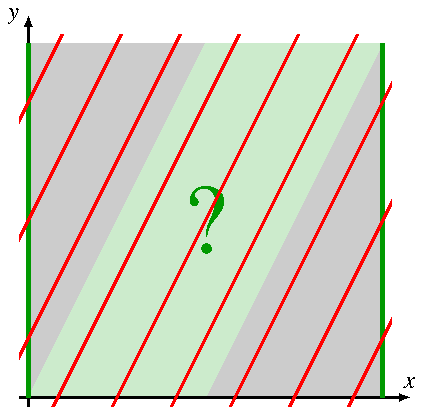
\includegraphics{3-geometry/images/underdetermined.pdf}
\end{center}
\caption{Boundary values on the left and right side: solution
not determined in the light green portion of the domain.
\label{geometrie:charrand1}}
\end{figure}

\begin{figure}
\begin{center}
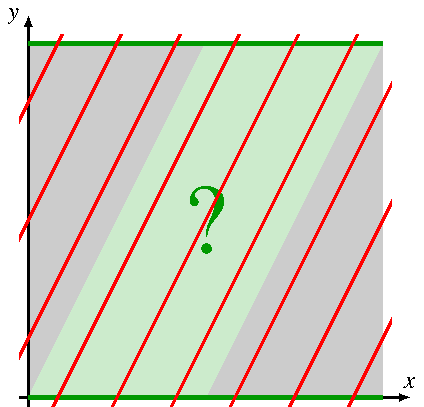
\includegraphics{3-geometry/images/overdetermined.pdf}
\end{center}
\caption{Boundary values on the top and bottom side of the square:
solution overdetermined in the light green portioin of the domain
\label{geometrie:charrand2}}
\end{figure}

\begin{figure}
\begin{center}
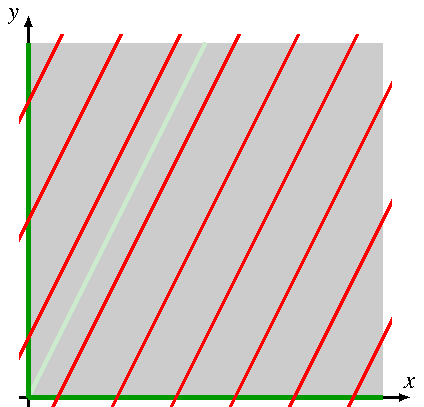
\includegraphics{3-geometry/images/nondifferentiable.pdf}
\end{center}
\caption{Boundary values on the left and bottom sides of the square:
solution well defined but differentiability on the light green
characteristic emanating from $(0,0)$ is not guaranteed.
\label{geometrie:charrand3}}
\end{figure}

\begin{figure}
\centering
\begin{tikzpicture}[>=latex]
\node at (0,0) {%
\includegraphics[width=0.9\hsize]{../common/3d/knick.jpg}%
};
\node at (7,-2.4) {$x$};
\node at (-7.2,-1) {$y$};
\node at (-3.7,3) {$z$};
\end{tikzpicture}
\caption{The solution of the differential
equation~(\ref{geometrie:knickbeispiel}),
with boundary values along the left and bottom sides of the square
(see also figure~\ref{geometrie:charrand3})
is not differentiable along the characteristic through $(0,0)$
(vertical axis scaled by a factor $0.4$).
\label{geometrie:knick}}
\end{figure}

As an illustration of the last case consider the boundary values
\begin{align*}
u(x_0,0)&=0,\\
u(0,y_0)&=y_0.
\end{align*}
Each side fixes part of the solution in the unit square, we can get 
explicit formulas using the method of characteristics.
The characteristics starting from the bottom side are
\[
\left.
\begin{aligned}
x&=x_0+t\\
y&=2t\\
u&=3t
\end{aligned}
\right\}
\qquad\Rightarrow\qquad
\left\{
\begin{aligned}
t&=\frac12y\\
u&=\frac32y
\end{aligned}
\right.
\]
The characteristics from the left side of the square are
\[
\left.
\begin{aligned}
x&=t\\
y&=y_0+2t\\
u&=y_0+3t
\end{aligned}
\right\}
\qquad\Rightarrow\qquad
\left\{
\begin{aligned}
y_0&=y-2x\\
u&=y+x
\end{aligned}
\right.
\]
Thus the solution function is
\[
u(x,y)=\begin{cases}
\frac32y&\qquad y<2x\\
x+y&\qquad y>2x,
\end{cases}
\]
as displayed in figure~\ref{geometrie:knick}.
For $y=2x$, both terms coincide, so the solution function is continuous
in all of $\Omega$.
However, the partial function $x\mapsto u(x,y)$ has slope $1$
for $y>2x$ and slope $0$ for $y<2x$, so it is not differentiable at $y=2x$.

